\documentclass[t]{beamer}
\usetheme{Copenhagen}
\setbeamertemplate{headline}{} % remove toc from headers
\beamertemplatenavigationsymbolsempty

\usepackage{amsmath, array, tikz, bm, pgfplots, tcolorbox, tkz-euclide}
\usetkzobj{all}
\pgfplotsset{compat = 1.16}

\title{Points, Lines, and Planes}
\author{}
\date{}

\AtBeginSection[]
{
  \begin{frame}
    \frametitle{Objectives}
    \tableofcontents[currentsection]
  \end{frame}
}

\begin{document}

\begin{frame} 
\maketitle
\end{frame}

\begin{frame}{Undefined Terms}
The \textbf{undefined terms} of geometry are \emph{point}, \emph{line}, and \emph{plane}. \newline\\	\pause

They are considered undefined because we can not give a definition for them without using other geometric terms. We can, at best, describe them.
\end{frame}

\begin{frame}{Points}
\textbf{Description:} a location without size.	\newline\\	\pause

We name a point using a dot with a capital letter.	\newline\\	\pause

\begin{center}
\begin{tikzpicture}
\tkzDefPoints{0/0/A}
\tkzDrawPoint[fill=black](A)
\tkzLabelPoints[right](A)
\end{tikzpicture}
\end{center}
\end{frame}

\begin{frame}{Lines}
\textbf{Description:} Straight path that extends in two opposite directions without end. \newline\\	\pause

A line contains an infinite number of points.	\newline\\	\pause

We name lines using 2 points with a capital letter, such as $\overleftrightarrow{AB}$ or $\overleftrightarrow{BA}$,	\newline\\	\pause

\begin{center}
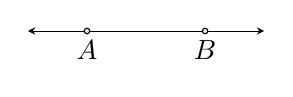
\begin{tikzpicture}
\tkzDefPoints{0.5/0/A, 2/0/B}
\tkzDrawSegment[add = 0.5 and 0.5, <->, >=stealth](A,B)
\tkzDrawPoints(A,B)
\tkzLabelPoints[below](A, B)
\end{tikzpicture}
\end{center}
\pause
or as a single lowercase letter such as $m$.
\begin{center}
\begin{tikzpicture}
\tkzDefPoints{0.5/0/A, 2/0/B}
\tkzDrawSegment[add = 0.5 and 0.5, <->, >=stealth](A,B)
\tkzDefPoints{2.7/0/m}    \tkzLabelPoints[right](m)
\end{tikzpicture}
\end{center}
\end{frame}

\begin{frame}{Planes}
\textbf{Description:} Flat surface that extends without end. \newline\\	\pause

A plane contains infinitely many lines.	\newline\\	\pause

We name a plane either by using a capital scripted letter such as $\mathcal{M}$, or by at least 3 points \underline{not on the same line} such as $ABC$.
\begin{center}
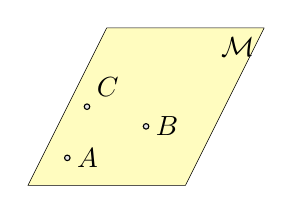
\begin{tikzpicture}
\tkzDefPoints{0/0/W, 2/0/Z, 1/2/X, 3/2/Y}
\tkzDrawPolygon[fill = yellow!25](W,X,Y,Z)
\tkzDefPoints{0.5/0.35/A, 1.5/0.75/B, 0.75/1/C}
\tkzLabelPoints[right](B)
\tkzLabelPoints[above right](C)
\tkzLabelPoints[right](A)
\tkzDrawPoints(A,B,C)
\tkzLabelPoint[below left](Y){$\mathcal{M}$}
\end{tikzpicture}
\end{center}
\end{frame}

\begin{frame}{Defined Terms Based on Undefined Terms}
Now that we have the undefined terms above, we can define other geometry vocabulary in terms of them.
\newline\\	\pause

\begin{tcolorbox}[colframe=green!20!black, colback = green!30!white,title=\textbf{Collinear Points}]
\textbf{Collinear points} are points that lie on the same line.
\end{tcolorbox}	\vspace{8pt}	\pause

\begin{center}
\begin{tikzpicture}[rotate=20]
\draw[<->,>=stealth] (-3,0) -- (3,0);
\draw[fill] (-2,0) circle [radius = 2pt] node [below] {$A$};
\draw[fill] (0,0) circle [radius = 2pt] node [below] {$B$};
\draw[fill] (2,0) circle [radius = 2pt] node [below] {$C$};
\end{tikzpicture}
\end{center}
\end{frame}

\begin{frame}{Coplanar Points}
\begin{tcolorbox}[colframe=green!20!black, colback = green!30!white,title=\textbf{Coplanar Points}]
\textbf{Coplanar points} are points and lines that lie on the same plane.
\end{tcolorbox}
\begin{center}
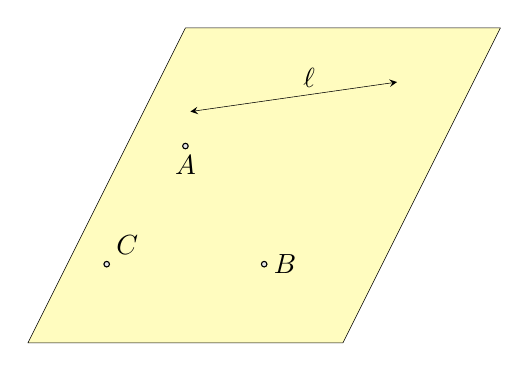
\begin{tikzpicture}
\tkzDefPoints{0/0/W, 4/0/Z, 2/4/X, 6/4/Y}
\tkzDrawPolygon[fill = yellow!25](W,X,Y,Z)
\tkzDefPoints{2/2.5/A, 3/1/B, 1/1/C, 2.5/3/D, 4.25/3.25/E}
\tkzLabelPoints[right](B)
\tkzLabelPoints[above right](C)
\tkzLabelPoints[below](A)
\tkzDrawPoints(A,B,C)
\tkzDrawSegment[add = 0.25 and 0.25, <->, >=stealth](D,E)
\tkzLabelSegment[above right](D,E){$\ell$}
\end{tikzpicture}
\end{center}
\end{frame}

\begin{frame}{Space}
\begin{tcolorbox}[colframe=green!20!black, colback = green!30!white,title=\textbf{Space}]
\textbf{Space} is the set of all points in 3 dimensions.
\end{tcolorbox}
\begin{center}
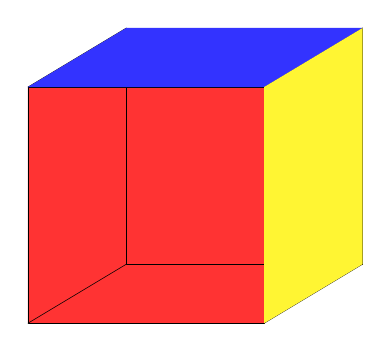
\begin{tikzpicture}
\tkzDefPoints{0/0/A, 3/0/B, 3/3/C, 0/3/D}
\tkzDrawPolygon[fill=red!80](A,B,C,D)
\tkzDefShiftPoint[A](1.25,0.75){E}
\tkzDefShiftPoint[B](1.25,0.75){F}
\tkzDefShiftPoint[C](1.25,0.75){G}
\tkzDefShiftPoint[D](1.25,0.75){H}
\tkzDrawPolygon(E,F,G,H)
\tkzDrawSegments(A,E B,F C,G D,H)
\tkzFillPolygon[blue!80](D,C,G,H)
\tkzFillPolygon[yellow!80](B,C,G,F)
\end{tikzpicture}
\end{center}
\end{frame}

\tikzset{
	ex1/.pic={
		\tkzDefPoints{0/0/A, 3.5/0/B, 1/2/C, 4.5/2/D}
		\tkzDrawPolygon(A,B,D,C)
		\tkzDefPoints{2/1/Q, 2/-0.5/N, 2/2.5/T, 1.35/1.35/R, 2.65/0.65/S, 3/1.5/W}
		\tkzDrawPoints(Q,N,T,R,S,W)
		\tkzLabelPoints[anchor = south west](Q,R,S,W)
		\tkzLabelPoints[left](N,T)
		\tkzDrawSegment[add = 0 and 0.25, ->, >=stealth](Q,T)
		\draw [dashed](Q) -- (2,0);
		\draw [->, >=stealth](2,0) -- (2,-1);
		\tkzDrawSegment[add = 0.35 and 0.35, <->, >=stealth](R,S)
		\node at (0.2,0) [anchor = south west] {$\mathcal{P}$};
		\node at (3.5,0.5) [anchor = east] {$\ell$};
	}
}

\begin{frame}{Example 1}
\begin{center}
\tikz \pic{ex1};
\end{center}
(a)	\quad What are two other ways to name $\overleftrightarrow{QT}$?	\newline\\
\onslide<2->{$\overleftrightarrow{QN}$ and $\overleftrightarrow{TN}$}
\end{frame}

\begin{frame}{Example 1}
\begin{center}
\tikz \pic{ex1};
\end{center}
(b) \quad What are two other ways to name $\mathcal{P}$?	\newline\\
\onslide<2->{plane $RQW$, plane $RSW$, and plane $QSW$}
\end{frame}

\begin{frame}{Example 1}
\begin{center}
\tikz \pic{ex1};
\end{center}
(c) \quad What are the names of 3 collinear points?	\newline\\
\onslide<2->{$R, \, Q, \text{ and } S$ \textbf{as well as} $T, \, Q, \text{ and } N$}
\end{frame}

\begin{frame}{Example 1}
\begin{center}
\tikz \pic{ex1};
\end{center}
(d) \quad What are the names of 4 coplanar points?	\newline\\
\onslide<2->{$R, \, Q, \, S, \text{ and } W$}
\end{frame}

\begin{frame}{Segments}
\begin{tcolorbox}[colframe=green!20!black, colback = green!30!white,title=\textbf{Segment}]
A \textbf{segment} is a part of a line that contains 2 endpoints and all points in between them.
\end{tcolorbox}
\vspace{8pt}	\pause

We name segments by the 2 endpoints such as $\overline{AB}$ or $\overline{BA}$.	\newline\\
\begin{center}
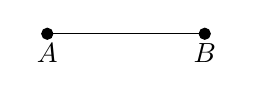
\begin{tikzpicture}
	\draw (0,0) -- (2,0);
	\draw[fill] (0,0) circle [radius=2pt] node [below] {$A$};
	\draw[fill] (2,0) circle [radius=2pt] node [below] {$B$};
\end{tikzpicture}
\end{center}
\end{frame}

\begin{frame}{Rays}
\begin{tcolorbox}[colframe=green!20!black, colback = green!30!white,title=\textbf{Ray}]
A \textbf{ray} is part of a line that consists of 1 endpoint and all the points on the line on one side of the endpoint.
\end{tcolorbox}
\vspace{8pt}	\pause

We name a ray by its endpoint and any point on the ray, such as $\overrightarrow{AB}$.
\begin{center}
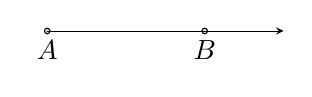
\begin{tikzpicture}
\tkzDefPoints{0/0/A, 2/0/B}
\tkzDrawPoints(A,B)
\tkzLabelPoints[below](A,B)
\tkzDrawSegment[->, >=stealth, add = 0 and 0.5](A,B)
\end{tikzpicture}
\end{center}
\onslide<3->{\emph{Note:} $\overrightarrow{AB}$ is not the same as $\overrightarrow{BA}$}
\end{frame}

\begin{frame}{Opposite Rays}
\begin{tcolorbox}[colframe=green!20!black, colback = green!30!white,title=\textbf{Opposite Rays}]
\textbf{Opposite rays} are two rays that share an endpoint and form a line.
\end{tcolorbox}
\vspace{8pt}	\pause

We name opposite rays by their shared endpoint and any point on each ray such as $\overrightarrow{CA}$ or $\overrightarrow{CB}$.	\newline\\
\begin{center}
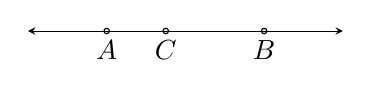
\begin{tikzpicture}
\tkzDefPoints{0/0/A, 2/0/B, 0.75/0/C}
\tkzDrawPoints(A,B,C)
\tkzLabelPoints[below](A,B,C)
\tkzDrawSegment[add = 0.5 and 0.5, <->, >=stealth](A,B)
\end{tikzpicture}
\end{center}
\end{frame}

\tikzset{
	ex2/.pic={
	\tkzDefPoints{0/0/D, 2/0/E, 3.5/0/F}
	\tkzDrawPoints(D,E,F)
	\tkzLabelPoints[below](D,E,F)
	\tkzDrawSegment[add = 0 and 0.25, ->, >=stealth](D,F)
	}
}

\begin{frame}{Example 2}
\begin{center}
	\tikz \pic{ex2};
\end{center}
(a)	\quad What are the names of the segments in the figure?	\newline\\	\pause
$\overline{DE}, \, \overline{ED}, \, \overline{DF}, \, \overline{FD}, \, \overline{EF}, \, \overline{FE}$	\newline\\	\pause
(b)	\quad What are the names of the rays in the figure?	\newline\\	\pause
$\overrightarrow{DE}, \, \overrightarrow{DF}, \, \overrightarrow{EF}$	\newline\\	\pause
(c)	\quad What are the names of the opposite rays?	\newline\\	\pause
There aren't any
\end{frame}

\begin{frame}{Postulates}
\begin{tcolorbox}[colframe=green!20!black, colback = green!30!white,title=\textbf{Postulates}]
A \textbf{postulate} (a.k.a. an \textbf{axiom}) is an accepted statement of fact.
\end{tcolorbox}
\vspace{6pt}	\pause
{\color{red}\textbf{Some Geometry Postulates:}}		\pause
\begin{itemize}
    \item Through any two points there is a line.	\pause
    \item If 2 different lines intersect, they intersect at a point.	\pause
    \item If 2 different planes intersect, they intersect at a line.	\pause
    \item You can draw a plane through any 3 noncollinear points.
\end{itemize}
\end{frame}

\begin{frame}{Example 3}

\end{frame}


\end{document}